\subsection{Modelos de S\'eries Temporais Univariados}\label{subsec:arima}

%A previsão de séries temporais é um desafio complexo, sem uma resposta fácil. 
%As séries temporais constituem na atualidade um tipo de estrutura de dados muito comum e frequente em diversas áreas da ciência, e sua análise continua sendo um grande desafio.
%As respostas às perguntas como: A bolsa de valores vai subir? Amanhã vai chover? Pode-se saber quando ocorrerá uma enchente? O valor do petróleo vai subir?, podem significar: redução de custo, maior lucro, menor prejuízo, melhor planejamento, melhoria de processos tornando seu estudo um grande atrativo.
%As séries temporais são conjuntos de observações de algum fenômeno, ordenados no tempo. Estas podem ser consideradas contínuas quando a coleta dos dados é realizada continuamente no tempo, e discretas quando a coleta desses dados é realizada em tempos específicos, geralmente equiespaçados. Além disso, a variável observada pode assumir valores discretos ou contínuos \cite{Martinho2023}.
%
%As abordagens de previsão de séries temporais existentes na literatura podem ser organizadas conforme \cite{Martinho2023}:
%técnicas Descritivas: consistem em analisar uma ou mais séries temporais através da representação e análise gráfica dos dados sequencialmente ao longo do tempo, o que pode revelar padrões de comportamento importantes: a tendência de crescimento (ou decrescimento), padrões cíclicos, alterações estruturais, observações aberrantes, entre outros;
%modelos lineares: incluem modelos probabilísticos, análise espectral, métodos não- paramétricos (alisamento ou suavização), modelos de espaço de estados, séries multivariadas, estudos longitudinais e processos de longa dependência;
%modelos não-lineares: englobam modelos não-lineares gerais (redes neurais artificiais, sistemas nebulosos, filtro de Kalman estendido, modelos híbridos), modelos pré-definidos, modelos com volatilidade variável, entre outros.

Os clássicos modelos do tipo ARIMA são compostos de três componentes: AR (Auto-Regressão), I (Integração) e MA (Média Móvel). O componente AR leva em consideração os valores anteriores da série temporal, o componente I trata das diferenças entre os valores observados para tornar a série estacionária, e o componente MA considera os erros residuais do modelo. Esses componentes combinados  tem por meta capturar os padrões e tendências presentes na série temporal.

\subsubsection{Componente Autorregressivo}

O componente auto-regressivo do modelo ARIMA é representado por AR$(p)$, em que o parâmetro $p$ determina o número de defesagens ou atrasos (do inglês \textit{lags}) a serem usados.
A equação do modelo AR$(p)$ é expressa da seguinte forma:

\begin{eqnarray}
	Y_t&=&c+\sum_{n=1}^{p} \alpha_n Y_{t-n} + \varepsilon_t\label{AR}
\end{eqnarray}


\noindent na equação \eqref{AR}, o termo $\varepsilon_t$ representa o ruído branco que é caracterizado por um sinal com média zero e variância sigma. Essa equação pode ser entendida como uma regressão múltipla, em que os valores defasados de $Y_t$ são utilizados como preditores. Esse modelo é conhecido como modelo autorregressivo de ordem $p$, ou AR$(p)$.


O modelo ARX é uma extensão do modelo AR, que incorpora variáveis exógenas nos dados para tentar melhorar as previsões. Esse modelo também é multivariado, e foi incluído aqui para fins de comparação com o modelo AR simples, considerando a presença de variáveis exógenas.


Pode-se mencionar que de acordo com o valor de $p$ tem-se alguns aspectos relevantes a citar:
Se o parâmetro $p$ for definido como zero AR($0$), significa que não há termos autorregressivos no modelo. Nesse caso, a série temporal se comporta como um ruído branco. 



\textbf{AR(1): Caminhadas aleat\'orias e Oscila\c c\~oes: }
Com o parâmetro $p$ definido como $1$, o modelo AR leva em consideração o valor anterior da série temporal multiplicado por um coeficiente e, em seguida, adiciona ruído branco. Quando o coeficiente é igual a $0$, há apenas ruído branco, resultando em uma série de tempo completamente aleatória, sem padrões previsíveis.

Quando o coeficiente é igual a $1$, ocorre uma caminhada aleatória, onde cada valor da série é obtido somando-se o valor anterior a um termo de ruído branco. Nesse caso, os valores da série apresentam uma tendência linear, aumentando ou diminuindo ao longo do tempo sem retornar à média.

Se o coeficiente estiver na faixa $0 < \alpha < 1$, ocorre o fenômeno de reversão média. Isso significa que os valores da série tendem a oscilar em torno de uma média central e a regressar em direção a ela após se afastarem. Esse padrão indica uma tendência de retorno à média ao longo do tempo.


\textbf{AR($p$): Termos de ordem superior: }
Aumentar ainda mais o parâmetro $p$ no modelo AR significa considerar um número crescente de medições de tempo anteriores, cada uma multiplicada pelo seu próprio coeficiente. Isso permite levar em conta uma memória mais longa da série temporal e capturar padrões de dependência complexos ao longo do tempo.

No entanto, é importante ter em mente que aumentar excessivamente o valor de $p$ pode levar a problemas de \textit{overfitting}, onde o modelo se ajusta muito bem aos dados de treinamento, mas tem um desempenho ruim na previsão de novos dados. Portanto, é necessário encontrar um equilíbrio entre a complexidade do modelo e sua capacidade de generalização.

%Além disso, é comum combinar o modelo AR com o modelo de média móvel (MA) para formar o modelo ARMA. O modelo MA considera os erros passados, ou seja, as diferenças entre os valores reais e as previsões anteriores, ajustadas por coeficientes. A combinação dos componentes AR e MA permite capturar tanto a dependência autorregressiva quanto a dependência na média móvel, proporcionando uma modelagem abrangente da série temporal.
%
%Em suma, aumentar o parâmetro $p$ no modelo AR pode melhorar a capacidade do modelo de capturar padrões complexos da série temporal, mas é necessário ter cuidado para evitar \textit{overfitting}. A combinação com o modelo MA pode fornecer uma modelagem mais completa dos dados. A escolha adequada dos parâmetros depende da análise cuidadosa dos padrões presentes na série temporal e do equilíbrio entre a complexidade do modelo e sua capacidade de generalização.

\subsubsection{M\'edia M\'ovel}\label{subsubsec:ma}
No modelo de média móvel (MA), o componente não é uma média móvel simples, mas sim uma combinação de termos de erro de previsão defasados. O parâmetro $q$ no modelo MA representa o número de termos de erro de previsão que são levados em consideração na previsão.

Este componente não é uma média móvel, mas sim os atrasos no ruído branco \cite{signal}.
Em um modelo MA(1), por exemplo, a previsão é composta por um termo constante, o produto do termo de erro de previsão anterior por um multiplicador, e o termo de erro de previsão atual. Essa abordagem baseia-se em princípios estatísticos e de probabilidade, ajustando a previsão com base em termos anteriores de erro de previsão.

O modelo MA é uma alternativa ao modelo AR e é usado para capturar padrões de dependência na média móvel, ou seja, a influência de erros passados na previsão atual. Ao combinar o modelo AR e o modelo MA, como no modelo ARMA, é possível obter uma modelagem mais abrangente que considera tanto a dependência autorregressiva quanto a dependência na média móvel \cite{arima}, tal que



\begin{eqnarray}
	y_t=c+\varepsilon_t+\theta_1 \varepsilon_{t-1}+\theta_2 \varepsilon_{t-2}+\cdots+\theta_q \varepsilon_{t-q}\label{eq:ma}
\end{eqnarray}

\noindent onde $\varepsilon_t$ representa o ruído branco, esse modelo é conhecido como um modelo de média móvel MA$(q)$, em que $q$ é a ordem da média móvel. É importante ressaltar que não se observam diretamente os valores de $\varepsilon_t$, portanto, essa modelagem não se trata de uma regressão no sentido convencional.

Diferentemente de uma regressão comum em que se têm variáveis explicativas observadas, no modelo MA$(q)$, são usados os termos de ruído branco defasados para estimar e prever os valores da série temporal. O objetivo é capturar a dependência dos termos de erro passados na previsão atual \cite{arima}.

%Esse modelo é útil para modelar séries temporais em que a média móvel tem um impacto significativo nas observações. Ao ajustar a série temporal com base nos termos de ruído branco defasados, pode-se obter uma estimativa dos valores futuros.
%
%Embora o modelo MA$(q)$ seja diferente de uma regressão tradicional, é uma ferramenta estatística para modelar e prever séries temporais, levando em consideração a dependência entre os termos de erro passados.


\subsubsection{Modelos ARMA e ARIMA}\label{subsubsec:arma}

O modelo ARMA é uma combinação dos modelos AR  e MA, onde o modelo AR é adicionado ao modelo MA.
No modelo ARMA, é adicionada uma constante à soma dos termos autorregressivos multiplicados pelos seus coeficientes, juntamente com a soma dos termos de média móvel multiplicados pelos seus coeficientes, além do ruído branco. Essa estrutura é amplamente utilizada em diversos modelos de previsão em diferentes áreas.
Esse modelo é bastante semelhante ao modelo ARIMA, pois calcula os termos, mas não inclui a diferenciação presente tanto no modelo ARMA quanto no modelo ARIMA, tal que

\begin{eqnarray}
	Y_t = \beta_2 + \omega_1\varepsilon_{t-1} + \omega_2 \varepsilon_{t-2} +\ldots+ \omega_q \varepsilon_{t-q} + \varepsilon_t \label{arima}
\end{eqnarray}

\noindent onde $Y_t$ representa a série temporal que foi diferenciada (possivelmente mais de uma vez). Os ``preditores'' no lado direito da equação incluem os valores defasados de $Y_t$ e os erros defasados. Esse tipo de modelo é conhecido como ARIMA ($p, d, q$).

O modelo ARIMA é uma extensão do modelo ARMA que incorpora uma etapa adicional de pré-processamento chamada de diferenciação. Essa etapa é representada pela notação I$(d)$, em que $d$ denota a ordem de diferenciação, ou seja, o número de transformações necessárias para tornar a série temporal estacionária. Portanto, um modelo ARIMA é simplesmente um modelo ARMA aplicado à série temporal diferenciada. Isso permite lidar com séries temporais que possuem tendências ou padrões não estacionários.

Embora os modelos ARIMA sejam eficazes, incorporar variáveis sazonais e exógenas ao modelo pode potencializar sua capacidade de previsão. No entanto, é importante destacar que o modelo ARIMA pressupõe que a série temporal seja estacionária. Quando lidamos com séries temporais não estacionárias, é necessário recorrer a outros modelos para a análise e previsão adequadas  \cite{arima}. Um exemplo é o do modelo SARIMA gerado por



\begin{eqnarray}
	Y_t&=&c+\sum_{n=1}^p \alpha_n y_{t-n}+\sum_{n=1}^q \theta_n \epsilon_{t-n}+\sum_{n=1}^P \phi_n y_{t-s n}+\sum_{n=1}^Q \eta_n \epsilon_{t-s n}+\epsilon_t \label{sarima}
\end{eqnarray}

O modelo proposto é uma extensão do modelo ARIMA, com a adição de componentes autorregressivos e de média móvel sazonal. Esses componentes extras são ajustados levando em consideração os padrões sazonais presentes nos dados, utilizando atrasos correspondentes à frequência sazonal (por exemplo, 12 para dados mensais). Essa abordagem permite capturar e modelar de forma mais precisa as variações sazonais e melhorar a qualidade das previsões em séries temporais com esse comportamento cíclico \cite{sarima}.

\subsection{Modelos de S\'erie Temporal Multivariada}\label{subsec:mult}

Os modelos de série temporal multivariada são uma abordagem estatística utilizada para analisar e prever dados que possuem múltiplas variáveis dependentes ao longo do tempo. Nesse tipo de modelo, considera-se a interdependência entre as diferentes séries temporais, permitindo a análise conjunta e a identificação de padrões e relações entre as variáveis. 

\textbf{ARIMAX e SARIMAX:}
Nesse modelo, são consideradas variáveis exógenas, ou seja, são utilizados dados externos para a realização das previsões. É importante ressaltar que mesmo que essas variáveis exógenas sejam indiretamente modeladas no histórico de previsões do modelo, ao incluí-las diretamente, o modelo será capaz de responder de forma ágil aos efeitos dessas variáveis  \cite{sarima}.

\begin{eqnarray}
	d_t=c+\sum_{n=1}^p \alpha_n d_{t-n}+\sum_{n=1}^q \theta_n \epsilon_{t-n}+\sum_{n=1}^r \beta_n x_{n_t}+\sum_{n=1}^P \phi_n d_{t-s n}+\sum_{n=1}^Q \eta_n \epsilon_{t-s n}+\epsilon_t \label{eq:sarmax}
\end{eqnarray}

$p$: Ordem de autorregressão de tendência (ACF)$-p$ é o número de termos autorregressivos (parte AR). Permite incorporar o efeito de valores passados em nosso modelo. Intuitivamente, isso seria semelhante a afirmar que é provável que esteja quente amanhã se tiver sido quente nos últimos 3 dias.

$d$: Diferença de tendência ordem$-d$ é o número de diferenças não sazonais necessárias para estacionariedade. Intuitivamente, isso seria semelhante a afirmar que é provável que seja a mesma temperatura amanhã se a diferença de temperatura nos últimos três dias tiver sido muito pequena.

$q$: Ordem da média móvel de tendência. (PCAF)$-q$ é o número de erros de previsão defasados na equação de previsão (parte MA). Isso nos permite definir o erro do nosso modelo como uma combinação linear dos valores de erro observados em momentos anteriores no passado.

Elementos sazonais em SARIMAX:

P: Ordem autorregressiva sazonal,
D: Ordem das diferenças sazonais,
P: Ordem de média móvel sazonal,
M: O número de etapas de tempo para um único período sazonal.
M é igual à defasagem ACF com o valor mais alto (normalmente em uma defasagem alta).
$D=1$ se a série tiver um padrão sazonal estável ao longo do tempo,
$D=0$ se a série tiver um padrão sazonal instável ao longo do tempo,
$P\geq1$ se a FAC for positiva na defasagem M, senão $P=0$,
$Q\geq1$ se a ACF for negativa na defasagem M, caso contrário $Q=0$,
$X$ variável exógena.
Na Figura \ref{fig:sarimaxmap} é mostrado como o modelo SARIMAX se comporta.


\begin{figure}[H]
	\centering
	\caption{Significado do modelo SARIMAX}
	\label{fig:sarimaxmap}
	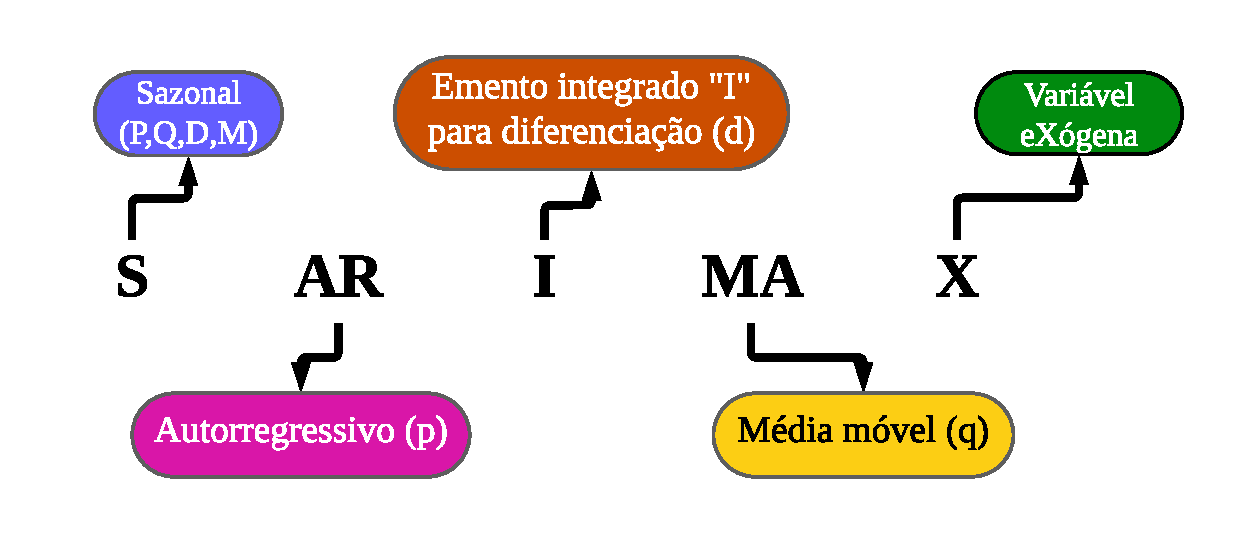
\includegraphics[width=0.7\linewidth]{Modelos/Figuras/sarimax_map}
	
\end{figure}

